\documentclass[12pt,a4paper]{article}
\usepackage{amsmath}
\usepackage{graphicx}

\begin{document}

\title{Determination of Spring Constant Using Static and Dynamic Methods}
\author{Dr. Öğr. Gör. Ahmet Ağaoğlu}
\date{25.12.2024}
\maketitle

\section*{Objective}
To calculate the spring constant \( k \) of a vertically hanging spring using two different methods: \textbf{static} and \textbf{dynamic}, and compare the results with error analysis.

\section*{Part 1: Static Method}

\subsection*{Setup}
\begin{itemize}
    \item Use a spring vertically suspended from a fixed support.
    \item Attach a mass of \( M = \text{xxx} \, \text{grams} \) to the free end of the spring.
\end{itemize}

\subsection*{Procedure}
\begin{enumerate}
    \item Record the initial position of the spring without any mass attached by taking a photo.
    \item Attach the mass \( M \) to the spring and allow it to settle into equilibrium.
    \item Record the final position of the spring by taking another photo.
\end{enumerate}
\begin{figure}
    \centering
    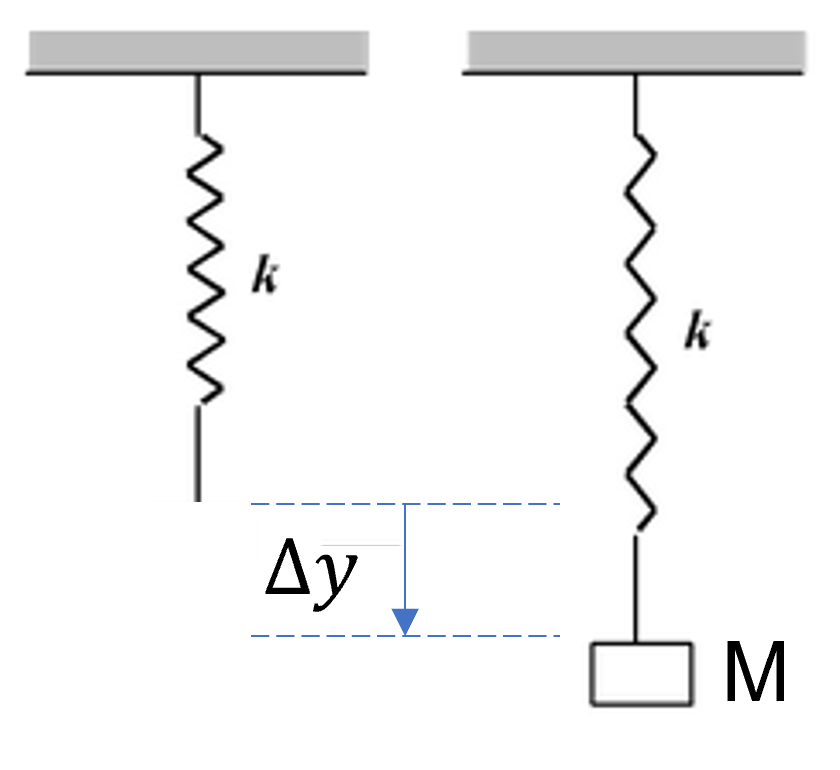
\includegraphics[width=0.35\linewidth]{static.png}
    \caption{Measurement of the elongation of the spring in the static setup.}
    \label{fig:static}
\end{figure}
\subsection*{Measurement}
\begin{itemize}
    \item Use the ruler provided on the setup to measure the displacement of the spring \( \Delta y \) from the photos, see Figure \ref{fig:static}.
    \item Calculate the weight \( W \) of the mass:
    \[
    W = M g
    \]
    where \( g = 9.81 \, \text{m/s}^2 \) is the gravitational acceleration.
    \item Determine the spring constant \( k \) using the formula:
    \[
    k = \frac{W}{\Delta y}
    \]
\end{itemize}
\subsection*{Uncertainty Calculation}
By driving chatGPT with the following prompt or your own modified prompt, determine the mean expected stiffness and it's uncertainty 
\begin{quote}
    \texttt{Propose a method to evaluate the stiffness of a spring by using photos of its initial and deflected states under a static load, with no more than 10 samples from each state, with results including histograms, the mean and standard deviations of deflections, the expected stiffness value and it's uncertainty.}
\end{quote}
Record chatGPT's response, and report it along with the prompt for future reference. If not sure about the meaning of an expected value and it's uncertainty, please ask chatGPT to define them for you. 

\section*{Part 2: Dynamic Method}

\subsection*{Setup}
\begin{itemize}
    \item Use the same spring-mass system.
    \item Attach a different mass \( m = \text{xxx} \, \text{grams} \) to the spring.
\end{itemize}

\subsection*{Procedure}
\begin{enumerate}
    \item Pull the mass down slightly to stretch the spring and then release it to initiate vertical oscillation.
    \item Record the motion of the oscillating mass using a video camera.
\end{enumerate}

\subsection*{Video Analysis}
\begin{itemize}
    \item Use the \textbf{Tracker Video Analysis Tool}: \texttt{https://physlets.org/tracker/}.
    \item Analyze the video to obtain the position-time graph of the mass's vertical motion.
\end{itemize}

\subsection*{Calculation}
\begin{itemize}
    \item Identify the period of the oscillation for the first two complete cycles \( T_1 \) and \( T_2 \), see Figure \ref{fig:dynamic}.
    \begin{figure}
        \centering
        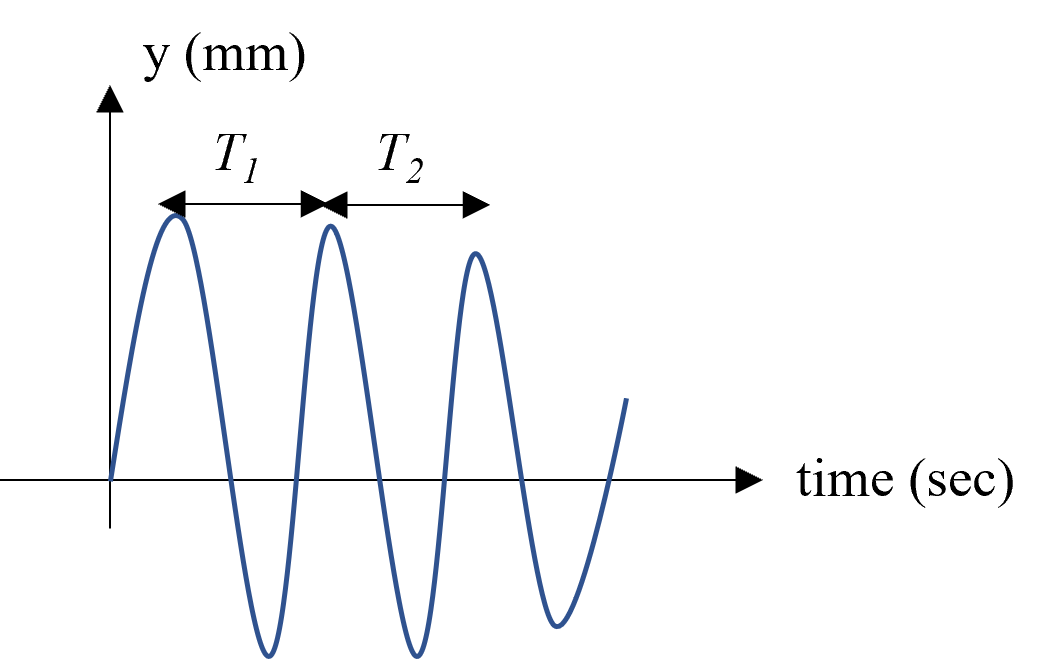
\includegraphics[width=0.5\linewidth]{dynamic.png}
        \caption{Vertical oscillation of the spring-mass system recorded in the dynamic setup}
        \label{fig:dynamic}
    \end{figure}
    \item Use the formula to calculate the spring constant for each period:
    \[
    k = \frac{4\pi^2 m}{T^2}
    \]
    \item Calculate the average \( k_{\text{dynamic}} \) from the two values obtained.
\end{itemize}

\section*{Comparison and Error Analysis}

Compare the static spring constant \( k_{\text{static}} \) with the dynamic spring constant \( k_{\text{dynamic}} \). Use the following formula to calculate the relative error \( E \):
\[
E = \left| \frac{k_{\text{dynamic}} - k_{\text{static}}}{k_{\text{static}}} \right| \times 100
\]
Interpret the results and discuss potential sources of error (e.g., measurement inaccuracies, damping effects, or alignment issues).


\end{document}

